\begin{exercises} 

\item The functions $f(x)$ and $g(x)$ are defined in the table below.  Use these function
    values to answer the following questions.
    \begin{center}
        \begin{tabular}[h!]{|c||c|c|c|c|c|c|c|}
            \hline
            $x$   & $-3$ &$-2$ &$-1$ &$ 0$ &$ 1$ &$ 2$ & $3$ \\ \hline \hline
            $f(x)$& $ 3$ &$ 1$ &$-1$ &$-3$ &$-1$ &$ 1$ & $3$\\ \hline
            $g(x)$& $-2$ &$-1$ &$ 0$ &$ 1$ &$ 0$ &$ 1$ & $2$\\ \hline
        \end{tabular}
    \end{center}
        (a) $f(-3)$, \quad (b) $g(3)$, \quad (c) $f(g(-3))$, \quad (d) $g(f(3))$, \quad
        (e) $f(g(f(-3)))$ \\
        (f) Write a list of value of $f(-x)$ for $x = -3, -2, \dots, 2, 3$.  Based on
            this list is $f(x)$ an even function, an odd function, or neither?\\
        (g) Repeat part (f) for $g(x)$.
\begin{exerciseSolution}
\end{exerciseSolution}


\item Find the inverse of each of the following functions.  If necessary state a
    restriction on the domain of $f(x)$ so that the inverse actually exists.
    \ba
        \item $f(x) = (2x-3)^2$
        \item $g(x) = x^2 - 2x + 1$
    \ea
\begin{exerciseSolution}
\end{exerciseSolution}


\item The plot on the left shows the function $f(x)$ and the plot on the right shows $g(x)
    = Af(B(x-C))+D$.  Find the appropriate values of $A$, $B$, $C$, and $D$.
    \begin{center}
%         \begin{tikzpicture}[scale=\scl]
%             \draw[color=gray] (-3,-3) grid (3,3);
%             \draw[thick, black, <->] (-3,0) -- (3,0) node[anchor=west]{$x$};
%             \draw[thick, black, <->] (0,-3) -- (0,3) node[anchor=west]{$x$};
%             \draw[very thick, blue] (-2,2) -- (-1,-1) -- (0,1) -- (1,0) -- (2,1)
%             node[anchor=south]{$f(x)$}; 
%         \end{tikzpicture} 
%         \begin{tikzpicture}[scale=\scl]
%             \draw[color=gray] (-3,-3) grid (3,3);
%             \draw[thick, black, <->] (-3,0) -- (3,0) node[anchor=west]{$x$};
%             \draw[thick, black, <->] (0,-3) -- (0,3) node[anchor=west]{$x$};
%             \draw[very thick, red] (-3,0) -- (-2,3) -- (-1,1) -- (0,2) -- (1,1)
%             node[anchor=south west]{$g(x)$}; 
%         \end{tikzpicture}
        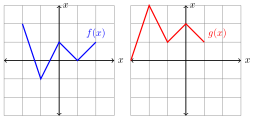
\includegraphics[width=0.7\columnwidth]{figures/0-3-fig7.pdf}
    \end{center}
\begin{exerciseSolution}
\end{exerciseSolution}

\item Use the function below to plot \\
    (a) $f(x)-3$, \quad (b) $f(x+1)$, \quad (c) $\frac{1}{2}f(x)$, \quad (d) $-f(x)$,
    \quad and (e) $\frac{1}{f(x)}$. 
    \begin{center}
%         \begin{tikzpicture}[scale=\scl]
%             \draw[color=gray] (-3,-3) grid (3,3);
%             \draw[thick, black, <->] (-3,0) -- (3,0) node[anchor=west]{$x$};
%             \draw[thick, black, <->] (0,-3) -- (0,3) node[anchor=west]{$x$};
%             \draw[very thick, blue] (-3,1) -- (-2,1) -- (0,0) -- (2,2) -- (3,2)
%             node[anchor=south]{$f(x)$}; 
%         \end{tikzpicture} 
%         \begin{tikzpicture}[scale=\scl]
%             \draw[color=gray] (-3,-3) grid (3,3);
%             \draw[thick, black, <->] (-3,0) -- (3,0) node[anchor=west]{$x$};
%             \draw[thick, black, <->] (0,-3) -- (0,3) node[anchor=west]{$x$};
%         \end{tikzpicture}
        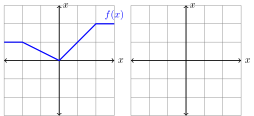
\includegraphics[width=0.7\columnwidth]{figures/0-3-fig8.pdf}
    \end{center}
\begin{exerciseSolution}
\end{exerciseSolution}


\end{exercises}
\afterexercises
